%\VignetteIndexEntry{DEGreport}
%\VignetteKeywords{DifferentialExpression, Visualization, RNASeq, ReportWriting}
%\VignetteEngine{knitr::knitr}

\documentclass{article}
\usepackage[utf8]{inputenc}




\RequirePackage[]{/Library/Frameworks/R.framework/Versions/3.4/Resources/library/BiocStyle/resources/tex/Bioconductor2}
\AtBeginDocument{\bibliographystyle{/Library/Frameworks/R.framework/Versions/3.4/Resources/library/BiocStyle/resources/tex/unsrturl}}


\title{DEGreport }
\author{Lorena Pantano}
\date{Modified: 2 July, 2016. Compiled: \today}

\begin{document}
maketitle
\tableofcontents
\newpage

\begin{knitrout}
\definecolor{shadecolor}{rgb}{0.941, 0.941, 0.941}\color{fgcolor}\begin{kframe}
\begin{alltt}
\hlkwd{library}\hlstd{(DEGreport)}
\hlkwd{data}\hlstd{(humanGender)}
\end{alltt}
\end{kframe}
\end{knitrout}

\section{General QC figures from DE analysis}

We are going to do a differential expression analysis with edgeR/DESeq2.
We have an object that is comming from the edgeR package. 
It countains a gene count matrix
for 85 TSI HapMap individuals, and the gender information. With that, we are 
going to apply the `glmFit` function or `DESeq2` to get genes differentially expressed 
between males and females.

\begin{knitrout}
\definecolor{shadecolor}{rgb}{0.941, 0.941, 0.941}\color{fgcolor}\begin{kframe}
\begin{alltt}
\hlkwd{library}\hlstd{(DESeq2)}
\hlstd{idx} \hlkwb{<-} \hlkwd{c}\hlstd{(}\hlnum{1}\hlopt{:}\hlnum{10}\hlstd{,} \hlnum{75}\hlopt{:}\hlnum{85}\hlstd{)}
\hlstd{dds} \hlkwb{<-} \hlkwd{DESeqDataSetFromMatrix}\hlstd{(}\hlkwd{assays}\hlstd{(humanGender)[[}\hlnum{1}\hlstd{]][}\hlnum{1}\hlopt{:}\hlnum{1000}\hlstd{, idx],}
                              \hlkwd{colData}\hlstd{(humanGender)[idx,],} \hlkwc{design}\hlstd{=}\hlopt{~}\hlstd{group)}
\hlstd{dds} \hlkwb{<-} \hlkwd{DESeq}\hlstd{(dds)}
\hlstd{res} \hlkwb{<-} \hlkwd{results}\hlstd{(dds)}
\end{alltt}
\end{kframe}
\end{knitrout}

We need to extract the experiment design data.frame where the condition is 
Male or Female.

\begin{knitrout}
\definecolor{shadecolor}{rgb}{0.941, 0.941, 0.941}\color{fgcolor}\begin{kframe}
\begin{alltt}
\hlstd{counts} \hlkwb{<-} \hlkwd{counts}\hlstd{(dds,} \hlkwc{normalized} \hlstd{=} \hlnum{TRUE}\hlstd{)}
\hlstd{design} \hlkwb{<-} \hlkwd{as.data.frame}\hlstd{(}\hlkwd{colData}\hlstd{(dds))}
\end{alltt}
\end{kframe}
\end{knitrout}

\subsection{Size factor QC}

A main assumption in library size factor calculation of edgeR and DESeq2 (and others)
is that the majority of genes remain unchanged. Plotting the distribution
of gene ratios between each gene and the average gene can show how true this is.
Not superuseful for many samples because the plot becomes crowed.

\begin{knitrout}
\definecolor{shadecolor}{rgb}{0.941, 0.941, 0.941}\color{fgcolor}\begin{kframe}
\begin{alltt}
\hlkwd{degCheckFactors}\hlstd{(counts[,} \hlnum{1}\hlopt{:}\hlnum{6}\hlstd{])}
\end{alltt}


{\ttfamily\noindent\color{warningcolor}{\#\# Warning: Removed 7 rows containing non-finite values (stat\_bin).}}\end{kframe}\begin{adjustwidth}{\fltoffset}{0mm}
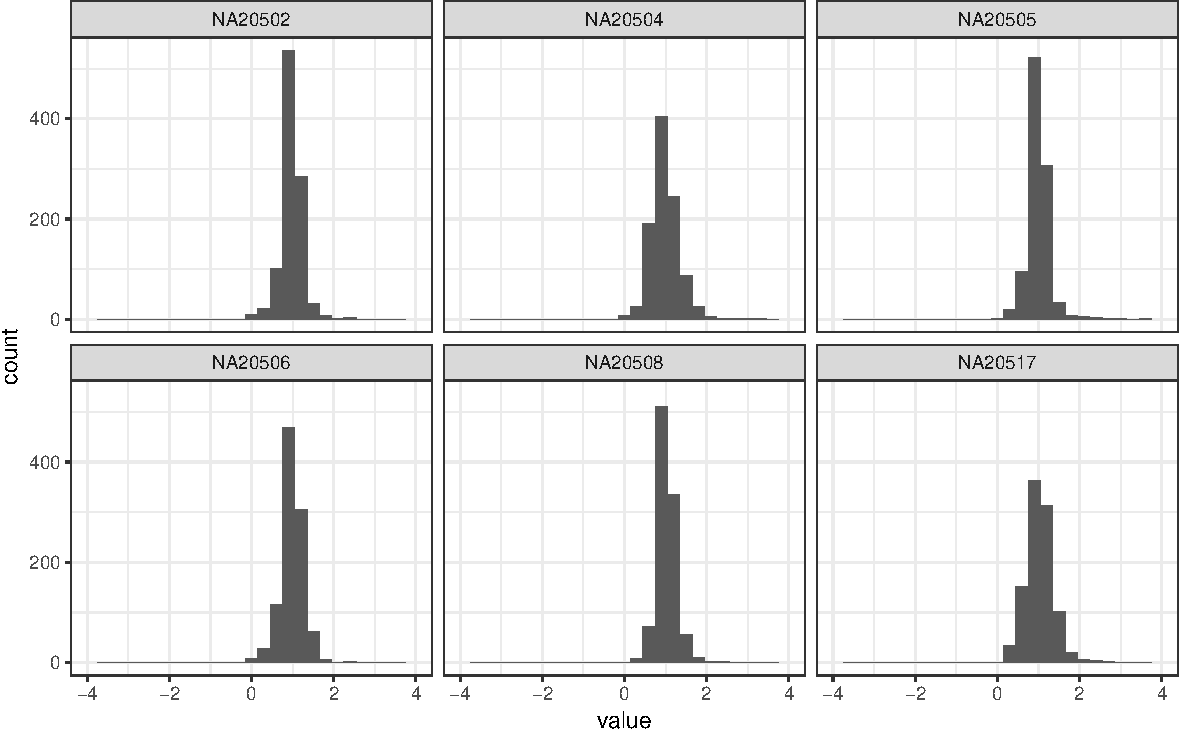
\includegraphics[width=\maxwidth]{figure/chunk-size-factor-1} \end{adjustwidth}
\end{knitrout}


\subsection{Mean-Variance QC plots}

p-value distribution gives an idea on how well you model is capturing the input data
and as well whether it could be some problem for some set of genes. In general,
you expect to have a flat distribution with peaks at 0 and 1. In this case, we add
the mean count information to check if any set of genes are enriched in any
specific p-value range.

Variation (dispersion) and average expresion relationship shouldn't be a factor among
the differentialy expressed genes. When plotting average mean and standard desviation,
significant genes should be randomly distributed.

In this case, it would be good to look at the ones that are totally outside the expected 
correlation.

You can put this tree plots together using \Rcode{degQC}.

\begin{knitrout}
\definecolor{shadecolor}{rgb}{0.941, 0.941, 0.941}\color{fgcolor}\begin{kframe}
\begin{alltt}
\hlkwd{degQC}\hlstd{(res[[}\hlstr{"pvalue"}\hlstd{]], counts, design[[}\hlstr{"group"}\hlstd{]])}
\end{alltt}
\end{kframe}
\end{knitrout}


\subsection{Covariates effect on count data}

Another important analysis to do if you have covariates is to calculcate
the correlation between PCs from PCA analysis to different variables you may
think are affecting the gene expression. This is a toy example of how the
function works with raw data, where clearly library size correlates with 
some of the PCs.

\begin{knitrout}
\definecolor{shadecolor}{rgb}{0.941, 0.941, 0.941}\color{fgcolor}\begin{kframe}
\begin{alltt}
\hlstd{resCov} \hlkwb{<-} \hlkwd{degCovariates}\hlstd{(}\hlkwd{log2}\hlstd{(}\hlkwd{counts}\hlstd{(dds)}\hlopt{+}\hlnum{0.5}\hlstd{),}
                        \hlkwd{colData}\hlstd{(dds))}
\end{alltt}
\end{kframe}\begin{adjustwidth}{\fltoffset}{0mm}
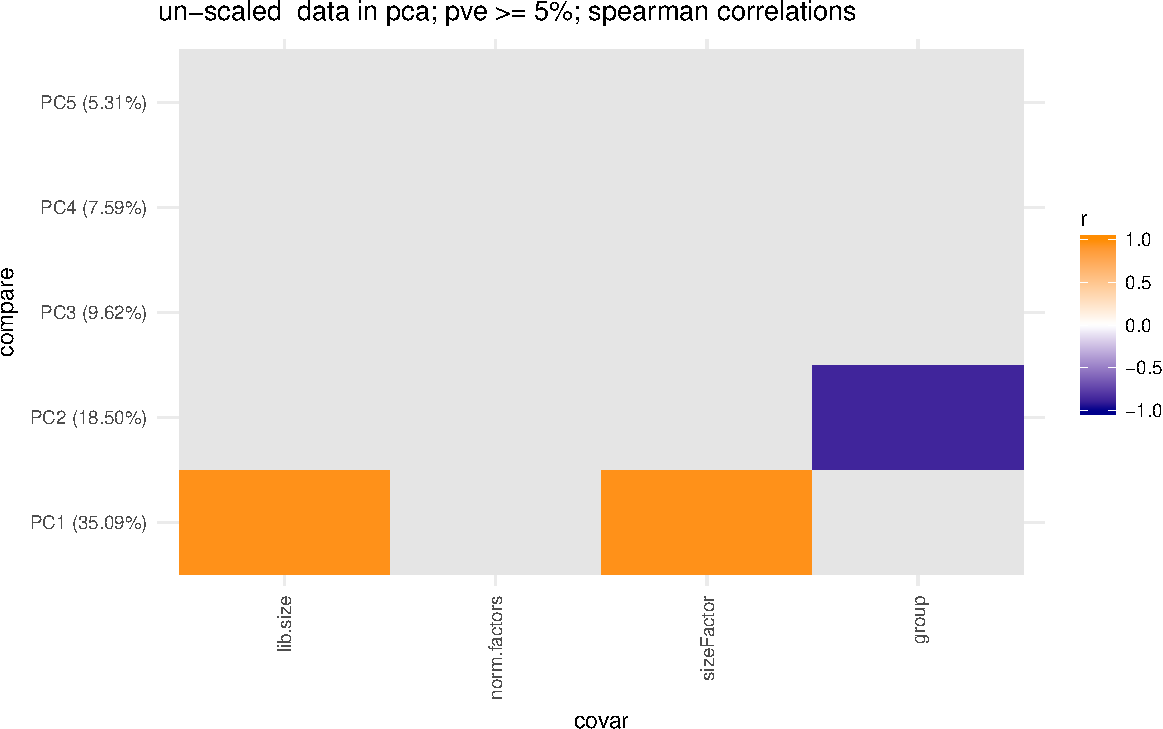
\includegraphics[width=\maxwidth]{figure/chunk-covariates-1} \end{adjustwidth}\begin{kframe}\begin{alltt}
\hlstd{resCov}\hlopt{$}\hlstd{plot}
\end{alltt}
\end{kframe}\begin{adjustwidth}{\fltoffset}{0mm}
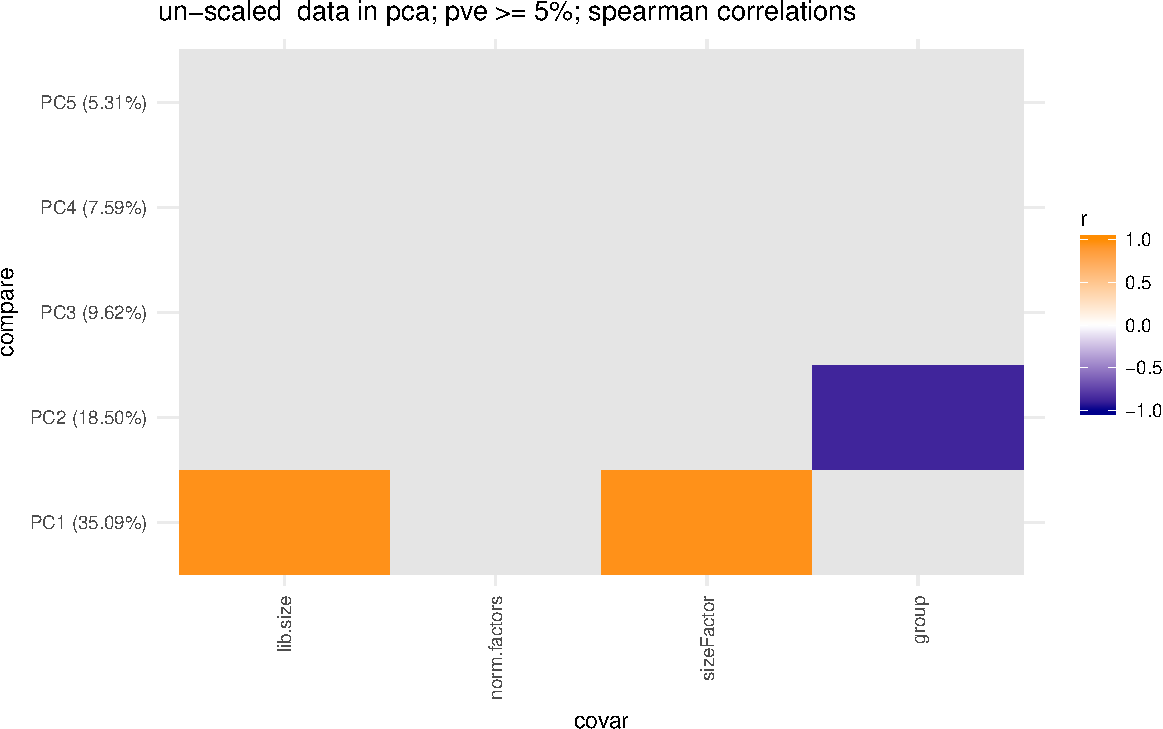
\includegraphics[width=\maxwidth]{figure/chunk-covariates-2} \end{adjustwidth}
\end{knitrout}


\subsection{Covariates correlation with metrics}

Also, the correlation among covariates and metrics from the analysis can
be tested. This is useful when the study has multiple variables, like in
clinical trials. The following code will return a correlation table, and
plot the correlation heatmap for all the covariates and metrics in a table.

















